\chapter{Apéndice}

En esta sección, se pueden encontrar diversos tipos de contenido, tales como datos brutos, códigos fuente, resultados detallados, diagramas extensivos, y cualquier otra documentación que, aunque esencial, podría interrumpir el flujo de lectura si se incluyera en el cuerpo principal del texto. El objetivo del apéndice es facilitar al lector interesado un acceso directo a estos materiales, permitiéndole profundizar en los aspectos técnicos o metodológicos del proyecto sin sobrecargar el texto principal.

\section{Circuitos}\label{ApendiceDiseñoEsquematico}

Los circuitos son una parte fundamental de cualquier proyecto de electrónica, y su correcto diseño y funcionamiento son esenciales para el éxito de la implementación. En esta sección, se incluyen los esquemáticos de los circuitos utilizados en el proyecto, así como cualquier información adicional relevante para su comprensión y reproducción.

Todos los circuitos que componen el proyecto se han originado de versiones anteriores de los mismos, y han sido adaptados y mejorados para cumplir con los requisitos específicos de la presente implementación.

\subsection{Esp32S3 con Agujero}\label{ApendiceEsp32Hole}
Dado que el componente ESP32S3 es un componente de montaje superficial y este posee una parte inferior con los pads de soldadura a tierra totalmente debajo del componente, se ha decidido modificar el componente (Parte de Eagle) para que sea más sencillo de soldar. Para ello, se ha añadido un agujero en la parte inferior del componente para que los pads de soldadura sean visibles desde el otro lado de la placa.

Para ello vamos a ir a Eagle e importaremos la librería de ESP32S3. Iremos a editar el \gls{Footprint} y donde están los terminales inferiores en mitad del dispositivo vamos a sustituirlos por un agujero de soldadura de las mismas dimensiones. 

Todos los pasos han sido realizados siguiendo el tutorial descrito en la asignatura de Circuitos Impresos. Una descripcion breve de los pasos a seguir es la siguiente.

\begin{enumerate}
    \item Abrir o Crear una Librería
    Abra EAGLE y cree una nueva librería con el nombre deseado (en nuestro caso, ``ESP32S3HOLE'').
    \item Seleccionar y Nombrar el Device
    Seleccione ``Device'' y asígnele un nombre (por ejemplo, ``ESP32S3HOLE'').
    \item Crear el Símbolo del Componente
    Dibuje el símbolo del componente y añada los pines necesarios, asignando nombres a cada pin según corresponda. Trace el diseño del símbolo de acuerdo con sus especificaciones. En nuestro caso podremos encontrar las dimenesiones, pines y demás en la hoja de datos del componente ESP32S3 \cite{ESP32S3Datasheet}.
    \item Usar un Package Existente
    Para ello, abra la librería en edición, vaya a la librería en el menú principal, elija el componente, haga clic con el botón derecho y seleccione la opción ``Copiar a Librería''.
    \item Editar el Footprint
    Abra la librería en edición, seleccione el componente, haga clic con el botón derecho y seleccione la opción ``Edit Package''. A continuación, edite el Footprint según sus especificaciones.
    Este paso es el más importante, ya que aquí es donde se añadirá el agujero de soldadura. Para ello, seleccione los pines inferiores del componente y sustitúyalos por un agujero de soldadura de las mismas dimensiones. Asegúrese de que el agujero de soldadura esté correctamente alineado con los pines del componente.
    Ahora que el Footprint ha sido modificado, guarde los cambios y cierre la ventana de edición.
    \item Unir Pines
    Para unir los pines del símbolo del componente con los pines del Footprint, seleccione el componente en la librería en edición, haga clic con el botón derecho y seleccione la opción ``Connect Package''.
    \item Añadir Atributos
    Añada los atributos necesarios al componente, como el valor, la descripción, etc.
\end{enumerate}

De forma que quedara como podemos ver en la figura \ref{fig:ESP32S3HOLE}.

\begin{figure}[H]
    \centering
    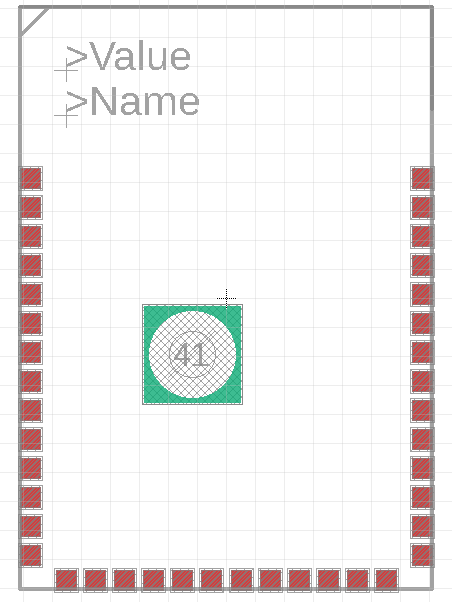
\includegraphics[width=0.7\textwidth]{imagenes/Capitulos/Cap13/ESP32S3HOLE.png}
    \caption{Imagen de la ESP32S3 modificada}
\end{figure}\label{fig:ESP32S3HOLE}

\section{PCB}\label{ApendicePCB}

\subsection{dimenesiones Fisicas}
Dado que el proyecto se va a realizar en una placa de madera, y esta contenga todos los elementos, y que la placa de madera va a ser fresada con una fresadora CNC, se ha decidido dejar margenes de 1mm en cada lado de la placa. Además de añadir un margen extra a la \gls{PCB} para que pueda ser atornillada más facilmente.

En la figura \ref{fig:PlanoSeparacionMadera} podemos ver en rojo el borde de la \gls{PCB} y la línea más próxima, en negro, la madera. Se ha dejado medio milímetro de margen para las máquinas \gls{CNC} y de fabricación de \gls{PCB}. Los marcadores de los interruptores generados por el software de la sección \ref{CreacionPlanoDistribucion} se ha dejado en verde.

\begin{figure}[H]
    \centering
    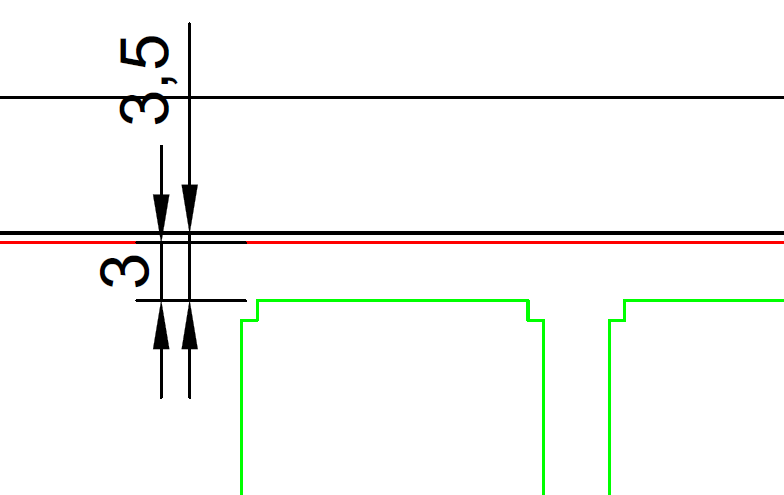
\includegraphics[width=0.8\textwidth]{imagenes/Capitulos/Cap05/AcotadoPCBMadera.png}
    \caption{Imagen del plano acotado del espacio entre las \glsnocase{Keycaps} y la madera.}
    \label{fig:PlanoSeparacionMadera}
\end{figure}

Tambien la idea siempre ha sido ajustar las dimensiones de la carcasa y \gls{PCB} para que no se viera la \gls{PCB} una vez que el teclado tuviese las \glsnocase{Keycaps} puestas, esto ya que al no haber \glsnocase{Plate} si dejaramos mucho hueco, esta parte se veria peor esteticamente. Por eso uno de los objetivos es intentar que la carcasa este lo más cerca de las \glsnocase{Keycaps}.
\newpage

\section{Programación}
\subsection{Codigo fuente}\label{ApendiceCodigoFuente}
\subsection{PID y VID}\label{ApendicePIDVID}
\subsection{Leds}\label{ApendiceLeds}
\subsection{Macros}\label{ApendiceMacros}

\section{Pruebas}\label{ApendicePruebas}
%Pruebas de programacion
Durante el desarrollo del proyecto, se han realizado diversas pruebas para verificar el correcto funcionamiento de los distintos componentes y módulos utilizados. Estas pruebas han sido fundamentales para identificar y corregir errores, así como para garantizar la calidad y fiabilidad del sistema final. En esta sección, se incluyen los detalles de las pruebas realizadas, así como los resultados obtenidos y las conclusiones derivadas de los mismos.

Durante todo el desarrollo se ha ido programando y probando el código en la placa de desarrollo ESP32S3. Se han realizado pruebas de los distintos componentes. El princpial modulo que se ha estado probando ha sido el modulo de la pantalla \gls{OLED} y el Multiplexor. La pantalla ha sido lo que más tiempo ha estado en desarrollo, ya que habia que hacer que funcionase con todos los estados del teclado. Asi mismo, esta tenia que ir cambiando de estado segun el estado del teclado. Por lo que cualquier error en las coordenadas o en la escritura de la pantalla se notaba facilmente y se podia corregir.

Para poder realizar la tarea de actualizar la pantalla se han ido ideando una serie de variables a lo largo del codigo que no indicarian donde esta el estado del teclado, asi podriamos desde cualquier parte del codigo saber en que estado se encuentra el teclado y poder actualizar la pantalla en consecuencia.

Dado que el entorno que teniamos para las pruebas no constaba de un teclado normal. Se decidio crear unas funciones de DEBUG que nos premitirian, mediante el serial de la placa de desarrollo, simular la pulsacion de las teclas. De esta forma podriamos probar el funcionamiento de la pantalla sin necesidad de tener un teclado conectado. Asi como el funcionamiento de la bateria, el bluetooth, etc. Y poder ir cambiando las variables de estado del teclado.

Como podemos ver en el codigo \ref{code:CodigoDebug} esta es la solucion que se ha optado y tambien se puede encontrar en el github del proyecto \cite{ModernWoodGitHub}. 

\begin{lstlisting}[style=console, language=bash, caption={Código de debug para la placa de desarrollo}, label={code:CodigoDebug}]
    #ifdef DEBUG
        // For debug purposes show how many times the loop is executed per second
        loop_counter++;
        if (millis() - last_loop_time > 1000)
        {
            Serial.print("Loop executed ");
            Serial.print(loop_counter);
            Serial.println(" times per second");

            Serial.print("Temperature: ");
            float result = 0;
            temp_sensor_read_celsius(&result);
            Serial.print(result);
            Serial.println(" C");

            loop_counter = 0;
            last_loop_time = millis();

            secs++;
            Serial.print("Seconds: ");
            Serial.println(secs);
        }

        // Read from serial
        char c = 'N';
        if (Serial.available())
        {
            c = Serial.read();
            Serial.print("Read from serial: ");
            Serial.println(c);
        }
        // wasd -> ARRIBA ABAJO DERECHA IZQUIERDA
        // Espace -> Enter
        // E -> Escape
        // Q -> MODO ESPECIAL
        switch (c)
        {
        case 'Q':
            WorkingAsKeyboard = !WorkingAsKeyboard;
            interrupted_FN = true;
            break;

        case 'E':
            MenuPressed[ArrEsc] = true;
            break;

        case ' ':
            MenuPressed[ArrEnter] = true;
            break;

        case 'W':
            MenuPressed[ArrUp] = true;
            break;

        case 'S':
            MenuPressed[ArrDown] = true;
            MenuPressed[ArrDown] = true;
            break;

        case 'A':
            MenuPressed[ArrLeft] = true;
            break;

        case 'D':
            MenuPressed[ArrRight] = true;
            break;

        case '1':
            batteryLevel--;
            batteryLevelChanged = true;
            break;

        case '2':
            batteryLevel++;
            batteryLevelChanged = true;
            break;

        case '3':
            connectionChanged = true;
            isUSBPreferred = !isUSBPreferred;
            isBLEPreferred = !isBLEPreferred;
            break;

        case '4':
            connectionChanged = true;
            isBLEConnected = !isBLEConnected;
            break;

        default:
            break;
        }

    #endif
\end{lstlisting}

\section{Ensamblaje}\label{ApendiceEnsamblaje}
\subsection{Errores}\label{ApendiceEnsamblajeErrores}

\section{Documentación}\label{ApendiceDocumentacion}
